%%%%%%%%%%%%%%%%%%%%%%%%%%%%%%%%%%%%%%%%%%%%%%%%%%%%%%%%%%%%%%%%%%%%%%
%
% Dario Palminio
%
% LaTeX Template: Curriculum Vitae
%
% Source: http://www.howtotex.com/
% Feel free to distribute this template, but please keep the
% referal to HowToTeX.com.
% Date: July 2011f
% 
%%%%%%%%%%%%%%%%%%%%%%%%%%%%%%%%%%%%%%%%%%%%%%%%%%%%%%%%%%%%%%%%%%%%%%
% How to use writeLaTeX: 
%
% You edit the source code here on the left, and the preview on the
% right shows you the result within a few seconds.
%
% Bookmark this page and share the URL with your co-authors. They can
% edit at the same time!
%
% You can upload figures, bibliographies, custom classes and
% styles using the files menu.
%
% If you're new to LaTeX, the wikibook is a great place to start:
% http://en.wikibooks.org/wiki/LaTeX
%
%%%%%%%%%%%%%%%%%%%%%%%%%%%%%%%%%%%%%%%%%%%%%%%%%%%%%%%%%%%%%%%%%%%%%%
\documentclass[paper=a4,fontsize=11pt]{scrartcl} % KOMA-article class
							
\usepackage[english]{babel}
\usepackage[utf8x]{inputenc}
\usepackage[protrusion=true,expansion=true]{microtype}
\usepackage{amsmath,amsfonts,amsthm}     % Math packages
\usepackage{graphicx}                    % Enable pdflatex
\usepackage[svgnames]{xcolor}            % Colors by their 'svgnames'
\usepackage{geometry}
	\textheight=700px                    % Saving trees ;-)
\usepackage{url}
\usepackage{hyperref}

\frenchspacing              % Better looking spacings after periods
\pagestyle{empty}           % No pagenumbers/headers/footers

%%% Custom sectioning (sectsty package)
%%% ------------------------------------------------------------
\usepackage{sectsty}

\sectionfont{%			            % Change font of \section command
	\usefont{OT1}{phv}{b}{n}%		% bch-b-n: CharterBT-Bold font
	\sectionrule{0pt}{0pt}{-5pt}{3pt}}

%%% Macros
%%% ------------------------------------------------------------
\newlength{\spacebox}
\settowidth{\spacebox}{8888888888}			% Box to align text
\newcommand{\sepspace}{\vspace*{1em}}		% Vertical space macro

\newcommand{\MyName}[1]{ % Name
		\Huge \usefont{OT1}{phv}{b}{n} \hfill #1
		\par \normalsize \normalfont}
		
\newcommand{\MySlogan}[1]{ % Slogan (optional)
		\large \usefont{OT1}{phv}{m}{n}\hfill \textit{#1}
		\par \normalsize \normalfont}

\newcommand{\NewPart}[1]{\section*{\uppercase{#1}}}

\newcommand{\PersonalEntry}[2]{
		\noindent\hangindent=2em\hangafter=0 % Indentation
		\parbox{\spacebox}{        % Box to align text
		\textit{#1}}		       % Entry name (birth, address, etc.)
		\hspace{1.5em} #2 \par}    % Entry value

\newcommand{\CertificatesEntry}[2]{      % Same as \CertificatesEntry
		\noindent\hangindent=2em\hangafter=0 % Indentation
		\parbox{\spacebox}{        % Box to align text
		\textit{#1}}			   % Entry name (birth, address, etc.)
		\hspace{1.5em} #2 \par}    % Entry value	
		
\newcommand{\SkillsEntry}[2]{      % Same as \PersonalEntry
		\noindent\hangindent=2em\hangafter=0 % Indentation
		\parbox{\spacebox}{        % Box to align text
		\textit{#1}}			   % Entry name (birth, address, etc.)
		\hspace{1.5em} #2 \par}    % Entry value	
		
\newcommand{\EducationEntry}[4]{
		\noindent \textbf{#1} \hfill      % Study
		\colorbox{Black}{%
			\parbox{6em}{%
			\hfill\color{White}#2}} \par  % Duration
		\noindent \textit{#3} \par        % School
		\noindent\hangindent=2em\hangafter=0 \small #4 % Description
		\normalsize \par}

\newcommand{\WorkEntry}[4]{				  % Same as \EducationEntry
		\noindent \textbf{#1} \hfill      % Jobname
		\colorbox{Black}{\color{White}#2} \par  % Duration
		\noindent \textit{#3} \par              % Company
		\noindent\hangindent=2em\hangafter=0 \small #4 % Description
		\normalsize \par}

		
\newcommand{\CoursesEntry}[4]{				  % Same as \EducationEntry
		\noindent \textbf{#1} \hfill      % Jobname
		\colorbox{Black}{\color{White}#2} \par  % Duration
		\noindent \textit{#3} \par              % Company
		\noindent\hangindent=2em\hangafter=0 \small #4 % Description
		\normalsize \par}
		
%%% Begin Document
%%% ------------------------------------------------------------
\begin{document}
% you can upload a photo and include it here...
%\begin{wrapfigure}{l}{0.5\textwidth}
%	\vspace*{-2em}
%		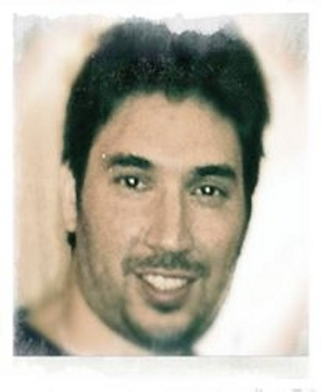
\includegraphics[width=0.15\textwidth]{photo}
%\end{wrapfigure}

%%% Photo
\begin{figure}
	\hfill
	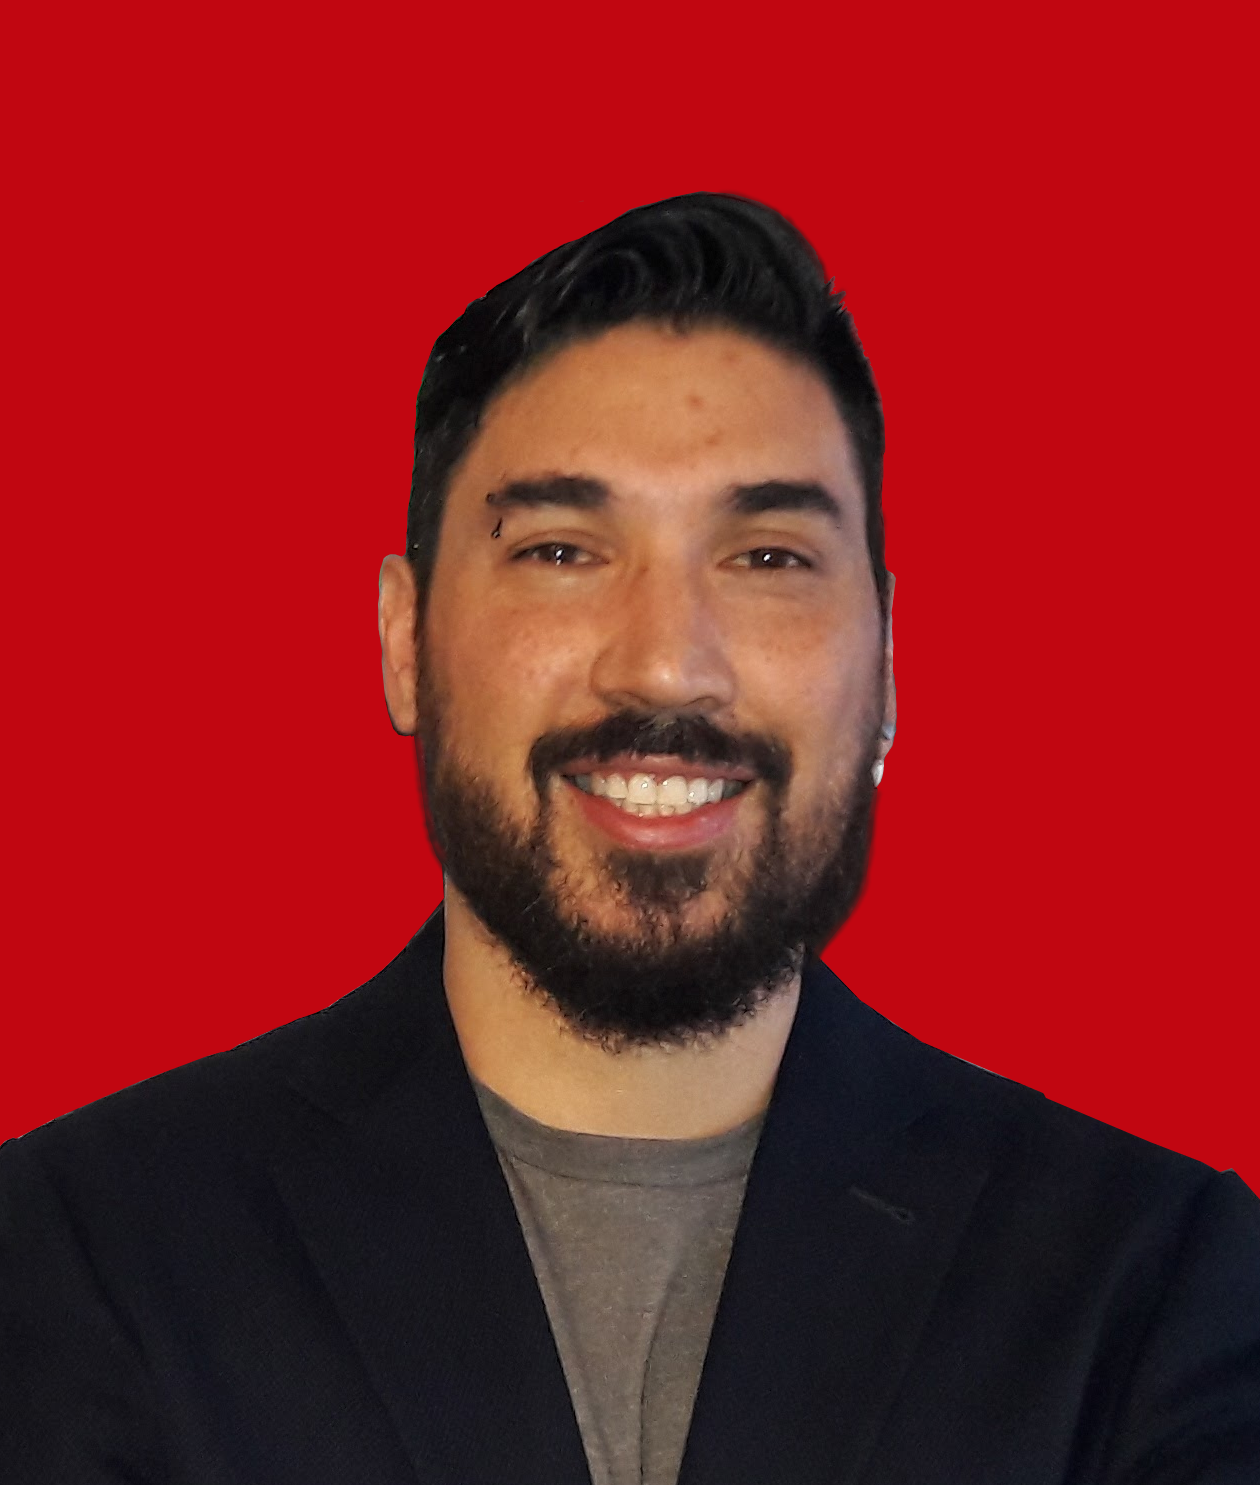
\includegraphics[width=0.2\textwidth]{photo1}
	\vspace{-7cm}
\end{figure}

%%% Title
\MyName{Dario Andrés Palminio}
\MySlogan{Curriculum Vitae}

\sepspace

%%% Personal details
%%% ------------------------------------------------------------
\NewPart{Datos personales}{}

\PersonalEntry{Nacimiento}{6 de Enero de 1977 en Rosario (Argentina)}
\PersonalEntry{Nacionalidad}{Argentino y Chileno nacionalizado}
\PersonalEntry{Localización}{Santiago de Chile}
\PersonalEntry{Teléfono}{(56) 979513358}
\PersonalEntry{Mail}{\url{dario.palminio  @  gmail.com}}
\PersonalEntry{linkedin}{\url{https://www.linkedin.com/in/palminio}}
\PersonalEntry{Sitio web}{\url{https://www.balancing-loop.com}}

%%% summary
%%% ------------------------------------------------------------
\NewPart{Sumario}{}

Soy un Ingeniero de Sistemas y entrenador y habilitador de agilidad con experiencia como Consultor, Agile Coach, Digital Transformation Advisor, Scrum Master Sr., Team Facilitator e Ingeniería de Software. Las aptitudes con las que me desenvuelvo son: pensador sistémico, liderazgo servicial, resiliente y mejorador, facilitador, comunicativo y sociable, conciencia situacional, asertivo, transparente, mediador y resolutor de conflictos, entusiasta, proactivo y con actitud de empoderamiento.
Me gusta ayudar con cambios organizacionales, habilitar agilidad en las organizaciones y desarrollar equipos ágiles de excelencia que apliquen prácticas de ingeniería de software. También me llevo bien con la idea de ser un despertador servicial, que influencia en los cambios culturales, desarrollo personal profesional y en hacer que las cosas pasen. Busco desarrollarme en la divulgación, entrenamiento y habilitación de las prácticas ágiles, en Agile Coaching, Ingeniería del Sistema Organizacional y en acompañamiento de transformaciones organizacionales. En esta vía he escrito un libro ("Scrum en ingeniería de software"), mantengo blogs (http://agilismoeningenieriadesoftware.blogspot.cl), participo en comunidades, dicto capacitaciones e influencio, como agente de cambio, en las organizaciones en las cuales me desenvuelvo. Soy un apasionado de lo que hago y me gusta mejorar cada día.



\sepspace

%%% Education
%%% ------------------------------------------------------------
\NewPart{Educación}{}

%2003 - Systems Engineer: School of Exact Sciences, UNPA-UACO National University. Graduated in 2003.
\EducationEntry{Ingeniero de Sistemas}{2003}{UNPA-UACO}
{Universidad Nacional de la Patagonia Austral - Unidad Académica Caleta Olivia}

Estudié Ingeniería de Sistemas (en UNPA-UACO de Argentina, Santa Cruz) por ser una disciplina amplia que incluye a ingeniería de software y la gestión organizacional. Esta profesión tiene un enfoque científico-técnico, interdisciplinario, organizacional y de pensamiento sistémico para la invención y utilización de técnicas dirigidas a la construcción, operación y mantenimiento de sistemas, incluyendo sistemas sociales empresariales, cibernéticos y sistemas hombre-máquina.
\sepspace

%2000, Analyst: University Analyst Programmer: School of Engineering, UNPSJB University National. Graduated in 2000.
\EducationEntry{Analista de Sistemas}{2000}{UNPSJB}
{University National de la Patagonia San Juan Bosco}

Antes de ser ingeniero, estudié Analista de Sistemas (en UNPSJB de Argentina, Chubut) por ser una especialización técnica que provee la capacidad de abstracción y de análisis de sistemas, incluyendo software, sistemas de información y dominio de problemas organizacionales. 
\sepspace

%1995, Electromechanical: Electromechanical technician: School ENET 1. Graduated in 1995.
\EducationEntry{Electromecánico}{1995}{ENET 1}
{Técnico mecánico eletricista}

Hice mi formación secundaria, de nivel medio, en una escuela de educación técnica (en ENET de Argentina, Chubut) donde me recibí de Electromecánico, una combinación de electricista, electrónico y mecánico. Esto me dio una base científico-técnica útil para abordar problemas desde una perspectiva científica y técnica.
\sepspace

%%% Work experience
%%% ------------------------------------------------------------
\NewPart{Experiencia laboral}{}

%2018 Cencosud Agile Coach by Balancing Loop Consulting SpA
\WorkEntry{Cencosud (Balancing Loop contractor)}{Feb. 2018}{Agile Coach, Digital Transformation Advisor}{
Agile Coach y Digital Transformation Advisor en Transformación Digital del conglomerados de retail en América Latina Cencosud (como consultor y proveedor independiente). Trabajando en el equipo de transformación digital en las oficinas de Cencosud (Santiago de Chile). Buscamos la reinvención de la organización, una nueva forma de ser y hacer, que involucra un cambio cultural, estratégico y tecnológico; con el objetivo de habilitar la agilidad y una manera de generar propuestas de valor que satisfagan y desafíen la experiencia de usuario de los clientes de Cencosud.
}

%2018 Fundador de Balancing Loop Consulting SpA
\WorkEntry{Balancing Loop}{Feb. 2018}{Emprendedor}{
Emprendedor y Fundador de Balancing Loop Consulting SpA (http://www.balancing-loop.com/) una empresa de consultoría y habilitación de agilidad organizacional.
}

%2017 Cencosud Agile Coach by Globant
\WorkEntry{Cencosud (Globant contractor)}{Nov. 2017}{Agile Coach}{
Agile Coach en Transformación Digital del conglomerados de retail en América Latina Cencosud (como consultor de Globant). Trabajando en el equipo de transformación digital en las oficinas de Cencosud (Santiago de Chile).
\begin{itemize}
\item Evaluación y acompañamiento en madurez de equipos ágiles.
\item Acompañamiento en el proceso de transformación Digital.
\item Capacitación de Equipos y Product Owners.
\end{itemize}
}

\sepspace

%2014-2015 Globant (globant.com) Software Engineer.
\WorkEntry{LATAM Airlines (Globant contractor)}{2015 - Oct. 2017}{ScrumMaster Sr., Team Facilitator y Agile Coach de equipos}
{Scrum Master en un proyecto para aerolínea LATAM Airlines contratado por Globant Company, trabajando en las oficinas de LATAM, con las siguientes responsabilidades principales:
\begin{itemize}
\item Ayudar al equipo empleando las prácticas Agile para cumplir con los compromisos de los proyectos digitales.
\item Construir un ambiente confiable y seguro para el equipo.
\item Evaluar la madurez del equipo facilitando su mejora a un ritmo sostenible.
\item Facilitar el debate, la toma de decisiones y la resolución de conflictos.
\item Ayudar a la comunicación interna y externa, mejorar la transparencia e irradiar información.
\item Ayudan a mejorar el trabajo del Product Owner, ayudando a encontrar maneras de mantener el Product Backlog y el Release Plan.
\item Buscar lograr que el equipo trabaje eficiéntemente bajo los valores ágiles.
\item Procurar que se desarrollen prácticas de ingeniería para lograr productos de calidad.
\item Prestar atención a la organización colaborando en comunidades, buscando cohesión organizacional, influenciando para la adopción del agilismo y para que se mejore la eficiencia organizacional.
\item Brindar capacitaciones y charlas, en diferentes eventos, relacionadas a la agilidad y a la Ingeniería de Software.
\item Ayudar a brindar información y colaborar con otras áreas de la organización comunicándose con PMO, áreas de DevOps y de gestión.
\item Colaborar con la gestión de riesgos, manejo de impedimentos y análisis de causa raíces.
\item Ayudar en el camino de carrera y al crecimiento profesional y personal a los integrantes del equipo.
\item Colaborar, reportar y ayudar a Agile Manegers a realizar actividades o desarrollos de soluciones transversales u organizacionales.
\end{itemize}

Los últimos meses estuve ejerciendo como Consultor, Agile Coaching y Team Facilitator para diferentes áreas dentro de la empresa Globant y LATAM.
}

\sepspace

%2014-2015 Globant (globant.com) Software Engineer.
\WorkEntry{Globant}{2015}{Technical Leader, Scrum Master, Team Facilitator}
{
\begin{itemize}
\item Scrum Master y Team Facilitator de equipos en LAN Airlines trabajando en las oficinas de Globant Company.
\item Scrum Master y Technical Lead en Perl/Java tecnologías para cuenta de LAN en empresa Globant. Las tecnologías usadas fueron: Perl (POO with Moose, cgi, Test::Moore, Template Toolkit), MySQL, Linux, SVN, Git-Svn, CSS3, HTML5, Eclipse (RSE, EPIC), Review Board, Jenkins, etc. The Java Technologies used was SOAP, RESTful/RESTEasy, Spring, Maven, Javascript with front-end using MVC (Backbone.js). Los proyectos fueron  relacionados a recolección de datos para envío a Google Analytic, gestión de promosiones y gestión de canje preferente de pasajes y usuarios Lanpass.
\item Focal point y Desarrollador Java en proyectos de cambio de pasajes con arquitectura SOA.
\end{itemize}
}

\sepspace

%2012-2014 IBA Entertainment limited as Software Engineer Freelancer.
\WorkEntry{IBA Entertainment limited}{2012-2014}{Software Engineer Freelancer}
{Trabajé en modalidad Freelancer (Monotributista) como Ingeniero de Software, bajo el marco de trabajo eXtreme Programming, para sistema de sportsbetting (Sitio Bet3000.com). Algunas tecnologías usadas: Perl 5, EmbPerl Object, Object Perl, JSON, RESTful, Mojolicious, Perl DBI. Desarrollo en el proyecto Bet3000 (www.bet3000.com) para la empresa International Betting Association.}

\sepspace

%2013-2014 Make IT Coop. As Associate, Secretary
\WorkEntry{Make IT Coop.}{2013-2014}{Associate, Secretary}{
Fui Socio fundador y Secretario en una Empresa Cooperativa llamada Make IT Coop. Este fue un emprendimiento colaborativo, iniciado en la ciudad de Córdoba (Argentina), con el objetivo de desarrollar software en diferentes tecnologías web y prestar servicio de consultoría informática.
}

\sepspace

%2008-2010 Motorola Mobility as Software Engineer.
\WorkEntry{Motorola Mobility}{2008-2010}{Software Engineer}
{Fui Ingeniero de Software en Motorola Mobility de Argentina S.A. (Córdoba, Arg.) en proyectos tipo PMI y otros bajo el marco de trabajo eXtreme Programming. Desarrollos aplicaciones Java (J2EE para dispositivos móviles para sistema de telecomunicaciones)}

\sepspace

%2008-2010 Motorola S.C.A (Contractor Vates) as Software Engineer.
\WorkEntry{Motorola S.C.A (Contractor Vates)}{2008-2010}{Software Engineer}
{Fui desarrollador Java (J2SE and J2EE para dispositivos móviles y sistema de telecomunicaciones) contratado por Vates para trabajar en las oficinas de Motorola.}

\sepspace

%2008 Vates (www.vates.com) as Systems Engineer.
\WorkEntry{Vates}{2008}{Systems Engineer}
{Trabajé en Vates como desarrollador Java para sistema de Gestión de Compras Municipal (Mendoza).}

\sepspace

%2007 Santex America S.A. (santexgroup.com) as Software Engineer: Java Developer.
\WorkEntry{Santex America S.A.}{2007}{Software Engineer, Java Developer}
{Trabaje en un proyecto de desarrollo de una aplicación Java para "Sistema de Gestión de Procesos de Negocio" bajo el marco de certificación CMMI nivel 2.}

\sepspace

%2007 AYI & Asociados (BADI S.R.L) as Software Engineer: Java Developer, Computer Consultant Java.
\WorkEntry{AYI and Asociados (BADI S.R.L)}{2007}{Software Engineer, Java Developer, Computer Consultant Java}
{1) Desarrollador Java (J2EE) y Oracle para proyecto de Tarjeta Naranja.
2) Capacitador de "Oracle 9i: Build J2EE Applications" en InMotion, Santiago de Chile (Chile);
3) Capacitador de "Oracle AS 10g: R3 Build J2EE Applications" en oficinas de Oracle, Buenos Aires (Arg.).
}

\sepspace

%2006 Informatic forensics – Tribunal third in Comodoro Rivadavia City: Informatic Forensics.
\WorkEntry{Tribunal tercero de Comodoro Rivadavia}{2006}{Informático Forense}{
Ejercí como Informático Forense para el tribunal tercero de Comodoro Rivadavia (Argentina. Chubut).}

\sepspace

%2004-2006 24 months in Municipality of Comodoro Rivadavia city, Systems Engineer Juridical Informatics, Technical Leader.
\WorkEntry{Municipalidad de Comodoro Rivadavia}{2004-2006}{Systems Engineer Juridical Informatics, Technical Leader}
{Fui Líder Técnico en Proyecto del “Digesto Legislativo Municipal” en Asesoría letrada de la Municipalidad de Comodoro Rivadavia. El proyecto lo desarrollamos con un equipo compuesto por una abogada, un conjunto de informáticos y yo; y constaba de crear una compilación digital ordenada de normas jurídicas (ordenanzas, resoluciones, decretos reglamentarios, etc.) de la municipalidad dictadas por intendencia y el Concejo Deliberante de la ciudad.
}

\sepspace

%2004-2005 Teacher Mathematic Teacher, Software Teacher, Computation Teacher.
\WorkEntry{Profesor}{2004-2005}{Teacher Mathematic Teacher, Software Teacher, Computation Teacher}
{He ejercido como Profesor en escuelas pçublicas y privadas de Argentina. Las materias que impartí fueron las siguientes: 
1- Computación I (Basic Informatic) - ISIS (Instituto terciario privado); 
2- Computación II (Aplicaciones de Software) - ISIS (Instituto terciario privado); 
3- Computación III (Linux y Windows Net) - ISIS (Instituto terciario privado); 
4- Profesor de Software: Adaptación al ambiente de trabajo en ENET 2 (Escuela Técnica); 
5- Profesor de Matemática de 8-EGB  (dos cursos)- Escuela 119 (C. R.); 
6- Profesor de Matemática de 9-EGB (dos cursos)- Escuela 119 (C. R.).
}

\sepspace

%2000-2003 - DeSoft Development of Software
\WorkEntry{DeSoft}{2000-2003}{Developer, Technical Leader}{
Trabajé como cofundador y asociado en un emprendimiento PYME de desarrollo de software. Me desenvolví como Analista, Desarrollador y Líder técnico en proyectos de desarrollo de software para empresas de terserización petrolera y máquinas viales (de la Patagonia Argentina).}

\sepspace

%%% Certifications
%%% ------------------------------------------------------------
\NewPart{Certificaciones}{}

Pienso que la profesión una la conduce, la mejora y fortalece, principalmente con la experiencia práctica, no con certificaciones. Las certificaciones constituyen una manera de capacitación que ayuda a entrar en un tema en particular. En esta vía he desarrollado algunas certificaciones:
\sepspace

\CertificatesEntry{\large{\textbf{ScrumMaster}}}{}
\CertificatesEntry{}{
Certified ScrumMaster por SCRUM ALLIANCE.\newline
Licencia: 000428099\newline
URL: \url{https://www.scrumalliance.org/community/profile/dpalminio}
}
\sepspace

\CertificatesEntry{\large{\textbf{AMC}}}{}
\CertificatesEntry{}{
SCRUMstudy Agile Master Certified.\newline
}
\sepspace

\CertificatesEntry{\large{\textbf{SDC}}}{}
\CertificatesEntry{}{
SCRUMstudy - Accreditation Body for Scrum and Agile.\newline
License: License 89793\newline
}
\sepspace

\CertificatesEntry{\large{\textbf{SMAC}}}{}
\CertificatesEntry{}{
Scrum Master Accredited Certification por International Scrum Institute.\newline
Licencia: 59173583922442\newline
URL: \url{http://www.scrum-institute.org/International_Scrum_Institute_Certificate_Validation_Tool.php}
}
\sepspace

\CertificatesEntry{\large{\textbf{SPOAC}}}{}
\CertificatesEntry{}{
Scrum Product Owner Accredited Certification por International Scrum Institute.\newline
Licencia: 92432962027378\newline
URL: \url{http://www.scrum-institute.org/International_Scrum_Institute_Certificate_Validation_Tool.php}
}
\sepspace

\CertificatesEntry{\large{\textbf{SC4JD}}}{}
\CertificatesEntry{}{
Scrum Certification for Java Developer por International Scrum Institute.\newline
Licencia: 96122926946263\newline
URL: \url{http://www.scrum-institute.org/International_Scrum_Institute_Certificate_Validation_Tool.php}
}
\sepspace

\CertificatesEntry{\large{\textbf{Leading SAFe}}}{}
\CertificatesEntry{}{
Leading SAFe en curso.\newline

}
\sepspace

%%% Courses
%%% ------------------------------------------------------------
\NewPart{Cursos de Gestión y Organización}{}

Para mejorar día a día, además de la experiencia en campo, soy autodidacta, por lo que leo bastante y estudio en forma independiente. A su vez he realizado diferentes capacitaciones y diplomados de los cuales doy cuenta de algunos a continuación:
\sepspace

\CoursesEntry{Gestión Ágil de Proyectos (PMI-ACP)}{2017}{Present License CER-R5LNG3F3-210777}{}
\CoursesEntry{Curso de Certified Scrum Master}{2015}{Kleer, Cba.-Arg.}{}
\CoursesEntry{Scrum Leader}{2015}{ValueInnova, Cba.-Arg.}{}
\CoursesEntry{Especialización en Project Management}{2010}{UTNFRBA, Bs.As.-Arg.}{}
\CoursesEntry{Carrera de Project Management}{2008}{IAAP, PMI, Bs.As.-Arg.}{}
\CoursesEntry{Estructuración de Proyectos PM01.}{2007}{IAAP, Bs.As.-Arg.}{}
\CoursesEntry{Creación de Cooperativas.}{2012}{INAES, Cba.-Arg.}{}

\sepspace

%%% Skills - Otras Experiencias y Conocimientos
%%% ------------------------------------------------------------
\NewPart{Otras Experiencias y Conocimientos}{}

\sepspace

\SkillsEntry{\textbf{Métodos}}{Métodos y marcos de trabajo como: Marco Scrum (Scrum.or), Método Kanban, Scrumban, Lean Startup.
}
\sepspace

\SkillsEntry{\textbf{Framework}}{Frameworks de escalamiento como: Scaled Agile Framework (SAFe for Lean Enterprises), LeSS Framework (Large Scale Scrum, LeSS), Disciplined Agile Framework  (DAD), Nexus, Scrum@Scale (Scrum.or).
}
\sepspace

\SkillsEntry{\textbf{Change Mgmt.}}{Métodos de gestión del cambio como: Change Management 3.0 (J. Appelo), Leading Change (J. Kotter), Retional Model (R. Ackoff), PDCA Model y SoPK (E. Deming), ADKAR Model (PROSCI), Toyota Kata y Kanban System.).
}
\sepspace

\SkillsEntry{\textbf{Management}}{Teorías de gestión: Management 2.0, Systemic Management y Management 3.0 (J. Appelo).).
}
\sepspace

\SkillsEntry{\textbf{Languages}}{Spanish (mother tongue)}
\SkillsEntry{}{English (level 2)}

\sepspace




%%% References
%%% ------------------------------------------------------------
\NewPart{Referencias}{}
Para más información ver el prefil en linkedin.
Última fecha de actualización: 21 de Octubre de 2018.
\sepspace

\end{document}
